
%
% use cases
%

\chapter{Use cases}
\label{chapter:use-cases}

\section{Demo Use Cases}
\label{chapter:use-case-demo}

A set of demonstration use cases has been created in order to test and evaluate the Geocluster implementation described in chapter \ref{chapter:architecture-implementation}. The set consists of one non-clustering map and 3 maps based on the different clustering algorithms. The demo use cases were configured using various Drupal modules and exported into code using the Features module\footnote{\url{http://drupal.org/project/features}}.

\begin{itemize}

\item \textbf{Geocluster Demo} show cases maps based on the two clustering algorithms provided by Geocluster module: PHP-based clustering and MySQL-based clustering and an additional map that doesn't use clustering at all. The article content type of a standard Drupal installation is extended by a Geofield-based place field for storing locations. For each map, a separate View is configured to provide a GeoJSON feed. A Leaflet map is then added on top of the feed by using the Leaflet GeoJSON module. Figure \ref{fig:geocluster-demo-site} illustrates a screenshot of a Geocluster Demo installation.

\item \textbf{Geocluster Demo Solr} adds a show case of the Solr-based clustering algorithm. It provides a setup based on Views GeoJSON and Leaflet GeoJSON similar to the Geocluster Demo feature. In addition, a Search API Server and Index configuration is added for indexing and querying the data using Apache Solr.  

\item \textbf{Geocluster Demo Content} is a sub-module that automatically imports a set of demo content for testing the Geocluster Demo and Geocluster Demo Solr features.

\end{itemize}

\begin{figure}[h]
  \begin{center}
    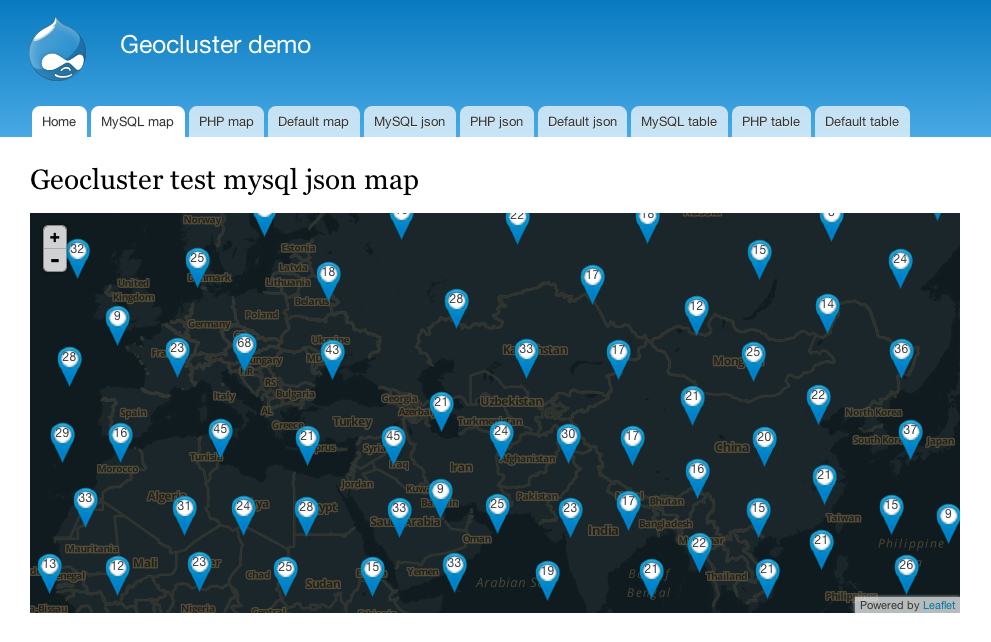
\includegraphics[width=1\textwidth]{figures/geocluster_demo_site.png}
    \caption{Screenshot of a Geocluster Demo installation. The active tab shows a map that uses MySQL-based clustering.}
    \label{fig:geocluster-demo-site}
  \end{center}
\end{figure}

\section{GeoRecruiter}
\label{chapter:use-case-georecruiter}

A practical use case for server-side geo clustering has been implemented for the Recruiter job board solution which has been introduced in chapter \ref{chapter:objective-use-cases}. It supports spatial search capabilities of the Recruiter distribution by visualizing a large amount of job offers on e-recruitment websites. GeoRecruiter allows to visualize several thousands of available jobs on an interactive map for large-scale e-recruitment websites. The Geocluster Solr module has been designed and used to provide the clustering capabilities needed by GeoRecruiter. The Solr-based aggregation integrates well with the architecture of the Recruiter distribution and is designed for scalability up to 1,000,000 indexed jobs as evaluated in chapter \ref{chapter:performance}. The prototype being discussed in the following chapter has been developed based on a copy of the Drupaljobs website\footnote{\url{http://drupaljobs.epiqo.com}}.

Drupaljobs is provided by epiqo as a show case for the Recruiter distribution. Its base features allow to create and search for job offers by companies as well as resumes of registered applicants on the e-recruitment platform. Figure \ref{fig:recruiter-job-search} depicts a screenshot of the heart of a Recruiter installation: the job search. The numbers on the figure indicate the main parts of such a page:

\begin{enumerate}

\item [(1)] A \textbf{search bar} above the content region.
\item [(2)] \textbf{Facetted filters} in the left sidebar.
\item [(3)] The \textbf{search results} as job teasers matching the search and filters.

\end{enumerate}

For scalability reasons, the job search functionality of Recruiter is based on Apache Solr using the Search API module which have been introduced in chapter \ref{chapter:data-storage}. The concept of using facetted filters, allows the site visitor to narrow down the result set by applying filters based on properties of the result set. The screenshot from figure \ref{fig:recruiter-job-search} displays filter facets based on \textit{organization}, \textit{fields of study} and \textit{occupational fields}. Every filter item indicates the number of results to be expected when using this particular filter. 

\begin{figure}[h]
  \begin{center}
    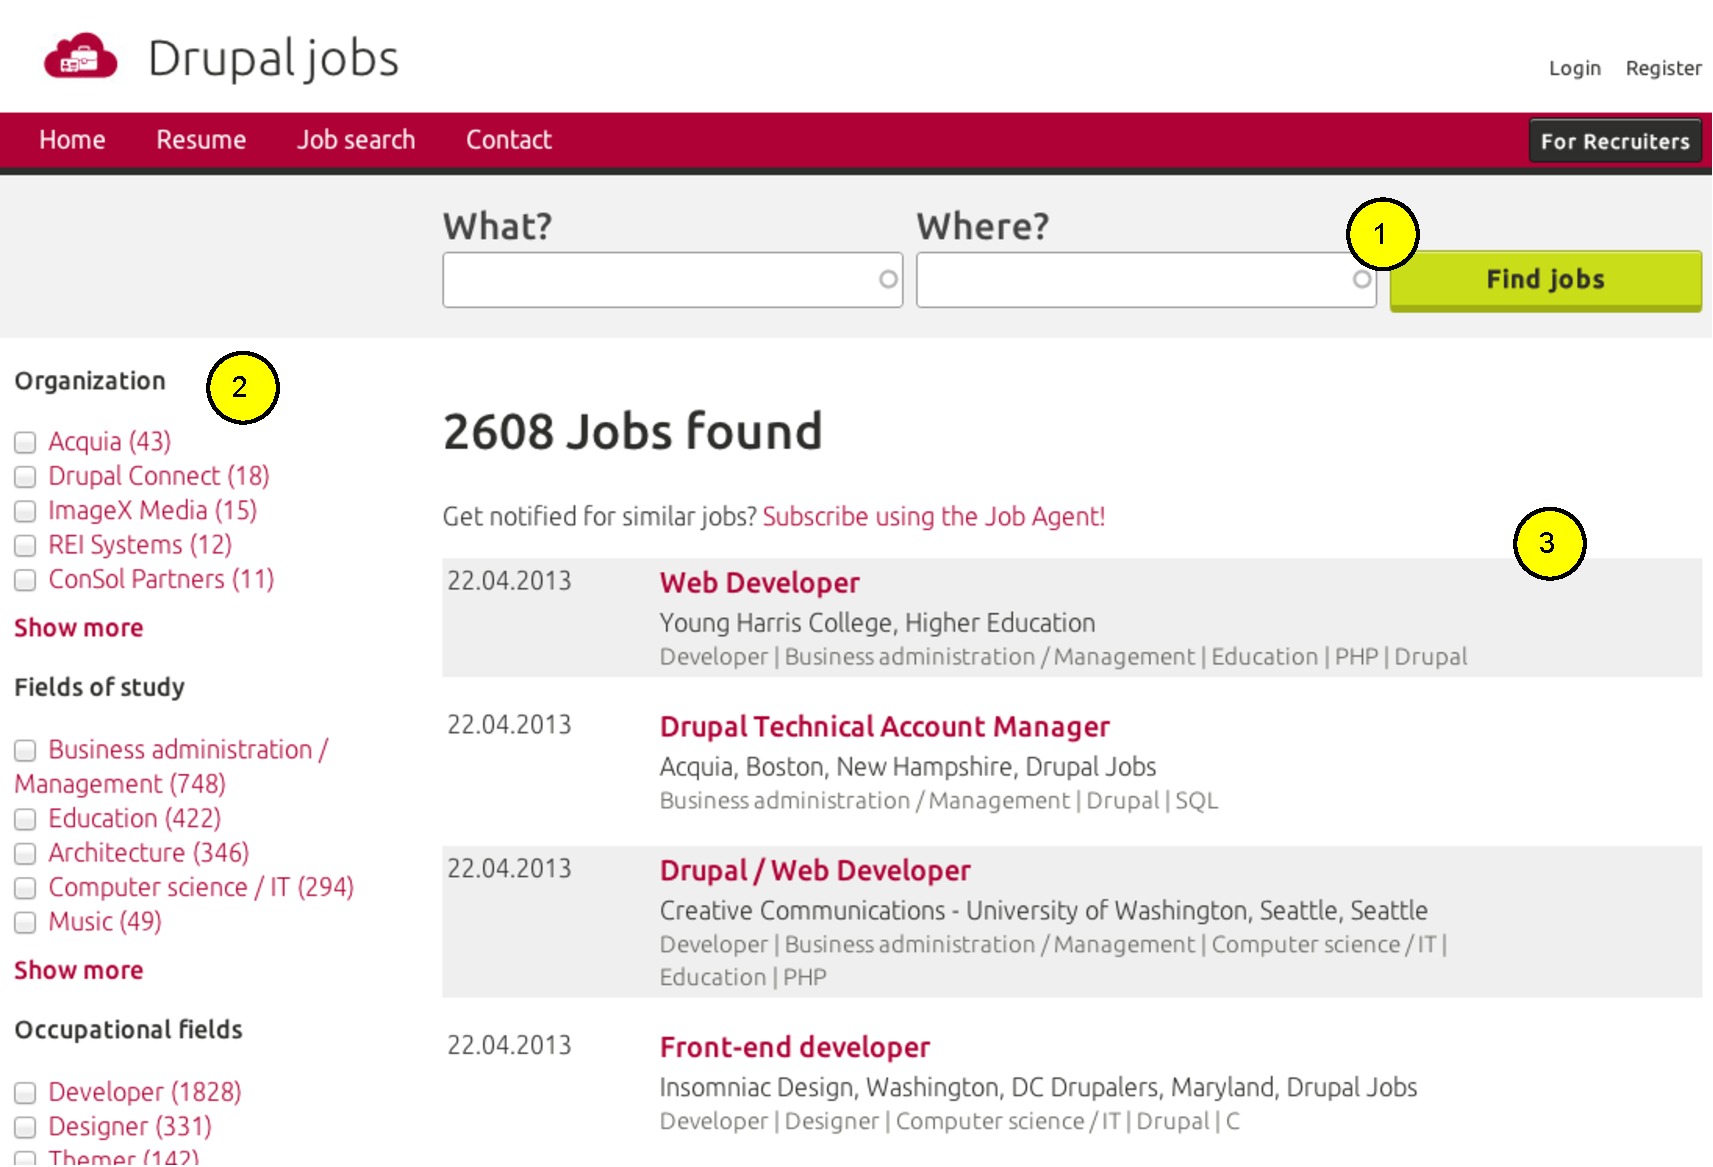
\includegraphics[width=1\textwidth]{figures/recruiter_job_search.pdf}
    \caption{Screenshot of a job search on Drupaljobs including indicators: (1) search bar, (2) facetted filters and (3) search results.}
    \label{fig:recruiter-job-search}
  \end{center}
\end{figure}

The GeoRecruiter use case consists of several geo-related additions to the Recruiter distribution. As previously stated, the customizations have been prototyped using a Drupaljobs test installation.

\begin{itemize}

\item \textbf{Add geospatial data}: The data model for posting job offers of the Recruiter distribution has been extended to support the annotation of a geospatial location as the \textit{place} property. In particular, a Geofield was added to the job node content types.

\item \textbf{Import test data}: Two sets of real-world geospatial test data have been prepared for the Drupaljobs test site. A set of 10,000 world-wide cities was created based on a dataset from GeoNames.org\footnote{\url{http://download.geonames.org/export/dump/cities1000.zip}}. Another set of 100,000 of U.S.-specific landmarks is based on a dataset from the U.S. Board on Geographic Names\footnote{\url{http://geonames.usgs.gov/docs/stategaz/NationalFile_20130404.zip}}. The kind of data isn't necessarily related to but will be mapped to job offers. This approach was taken due to the lack of a geospatially annotated datasets of job offers being available for testing purposes. Next, the test data was cleaned from errors and imported into the adapted Drupaljobs test installation. The import process was facilitated by using the Feeds module\footnote{\url{http://drupal.org/project/feeds}} which allows to import data into a Drupal site from external data sources like RSS feeds or in this particular case: CSV files.

\item \textbf{Configure Geocluster Solr}: The server-side clustering component explained in \ref{chapter:architecture-implementation} has been installed on the Drupaljobs test instance. The job search has been configured for clustering based on Apache Solr and Search API. Finally, a map visualizes the clustered job search results using Views GeoJSON and Leaflet. In order to enhance the representation of clusters and to experiment with interaction, the CSS styles of the client-side clustering library Leaflet.markercluster have been adapted and extended with additional colors for large clusters.

\item \textbf{Compare with client-side clustering}: In order to measure the effectiveness of the server-side clustering approach, a client-side clustering solution has been implemented for Drupaljobs as well. The client-side clustered map is based on a blog post by Ian Whitcomb of LevelTen~\cite{blog:leaflet-made-to-order}. For querying such a large dataset, he recommends circumnavigating the Views module and directly querying the database. The client-side clustering and visualization is again realized by the Leaflet.markercluster.

\end{itemize}

The resulting prototype allowed to experiment with the server-side clustering solution in a realistic environment, draw conclusions on effectiveness of clustering algorithm and the visualization component being used. A visualization of a map within the Drupaljobs test installation is provided in figure \ref{fig:drupaljobs-geocluster-solr}.

\begin{figure}[h]
  \begin{center}
    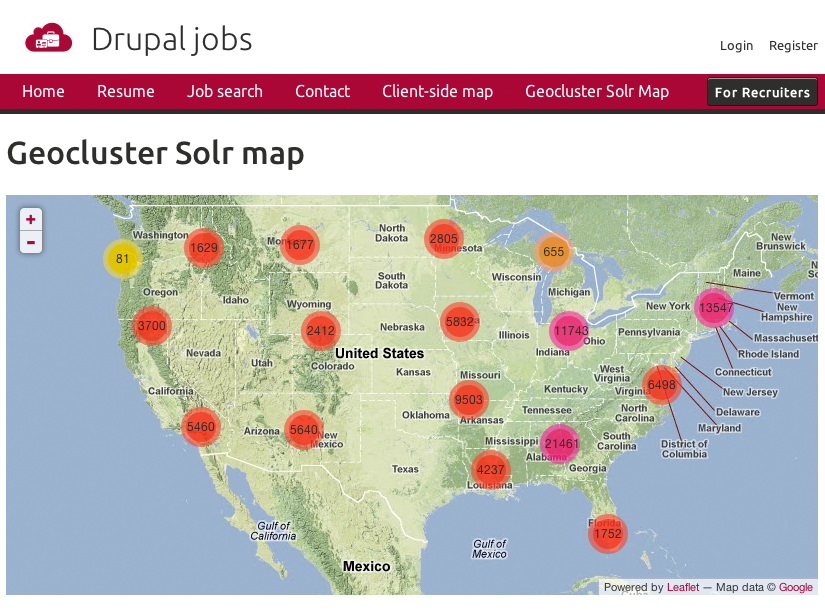
\includegraphics[width=1\textwidth]{figures/drupaljobs_geocluster_solr.png}
    \caption{Screenshot of map that visualized job search results on a map using Solr-based clustering on a Drupaljobs test installation.}
    \label{fig:drupaljobs-geocluster-solr}
  \end{center}
\end{figure}


Besides the clustering functionality, GeoRecruiter will support location-based search. This allows the user to search for jobs within the surroundings of a desired region by applying a proximity filter. The Search API Location module is currently being refactored\footnote{\url{http://drupal.org/node/1798168}} in order to provide a solid foundation for such spatial queries using Solr and the Search API module suite.








